\documentclass[12pt,english]{article}
\usepackage{mathptmx}

\usepackage{color}
\usepackage[dvipsnames]{xcolor}
\definecolor{darkblue}{RGB}{0.,0.,139.}

\usepackage[top=1in, bottom=1in, left=1in, right=1in]{geometry}

\usepackage{amsmath}
\usepackage{amstext}
\usepackage{amssymb}
\usepackage{setspace}
\doublespacing
\usepackage{lipsum}
\usepackage{indentfirst}
\usepackage{booktabs} 
\usepackage{threeparttable} 

\usepackage[authoryear]{natbib}
\usepackage{url}
\usepackage{booktabs}
\usepackage[flushleft]{threeparttable}
\usepackage{float}
\usepackage{graphicx}
\usepackage[english]{babel}
\usepackage{pdflscape}
\usepackage[unicode=true,pdfusetitle,
 bookmarks=true,bookmarksnumbered=false,bookmarksopen=false,
 breaklinks=true,pdfborder={0 0 0},backref=false,
 colorlinks,citecolor=black,filecolor=black,
 linkcolor=black,urlcolor=black]
 {hyperref}
\usepackage[all]{hypcap} 
\usepackage{breakurl}   
\bibliographystyle{jpe}



\linespread{2}

\begin{document}

\begin{singlespace}
\title{Pandemic Effects on Palm Beach County Real Estate}
\end{singlespace}

\author{Savannah J. Simpson\thanks{Department of Economics, University of Oklahoma.\
E-mail~address:~\href{mailto:student.name@ou.edu}{savannahjsimpson@ou.edu}}}

\date{May 6, 2024}

\maketitle

\begin{abstract}
The COVID-19 pandemic has significantly impacted the residential real estate market in Palm Beach County, Florida. This study aims to analyze the changes in housing prices and the influence of property characteristics on sale prices in two distinct municipalities, Jupiter and Boca Raton, before and after the pandemic. By comparing pre-COVID (2016-2019) and post-COVID (2021-2024) sales data, and applying a regression analysis, this study seeks to uncover the factors driving the surge in property values and assess the differential effects of the pandemic on these two markets. The findings reveal that while the relationship between property characteristics and sale prices strengthened in both municipalities following the pandemic, there were notable differences in the magnitude of these effects. This study contributes to a better understanding of the complex dynamics shaping the residential real estate market in the wake of the COVID-19 pandemic and provides valuable insights for homebuyers, investors, and policymakers in Palm Beach County.
\end{abstract}
\vfill{}


\pagebreak{}


\section{Introduction}\label{sec:intro}
\indent American industrialist, Henry Flagler, set the precedent for life in Palm Beach County with the completion of his Gilded Age mansion in 1902. Flagler, who is accredited with building the railroad that allowed the east coast of Florida to thrive, would be one of the first moguls to settle on Palm Beach Island, but certainly not the last. The Kennedy family would further bring light to life in Palm Beach with their lavish vacations and iconic style. The island has also been under controversy with the late Jeffery Epstein's infamous property being destructed, which is also just miles away from where Presidential Candidate Donald J. Trump resides at his Mar-A-Lago estate. Nonetheless, Palm Beach County has a rich culture of status and coastal living. 

While PBC is coined by a luxury island lifestyle, there are over a million residents who work, live, and lead on average lives on the other side of the bridge. While tourism is arguably one of the largest industries, not every Palm Beach resident leads the type of life that is highlighted in popular culture, and have to compete with visitors and transplants. This has always been a high-demand destination for vacation homes, but Florida would be overwhelmed with an influx of new dwellers following the global pandemic. The abundance of outdoor activities and more-than-lax COVID-19 restrictions held by Florida administrators became increasingly attractive to Northerners as they were cooped up in their city apartments. The real estate market as a whole has become convoluted since the pandemic for many reasons. Lifestyle adjustments have caused people's preferences to shift, and the increased popularity in remote work now allows professionals to contribute from any location. 

This societal phenomenon is particularly evident when assessing the housing market in Palm Beach County. Property values have exponentially risen across the United States, but have shown a prevalent skyrocket in southeast Florida. As discussed in The Palm Beach Post, county home prices have just hit a record high despite the expected summer real estate slow down. The average sale price of an existing, single family home in March of this year was \$1.19 million, showcasing a 32 percent increase from last year \cite{Miller2024}. Statistics such as these raise the question as to what is exactly going on behind the scenes of the real estate market. Is this a result of a volatile post-pandemic housing market, or is there something particular about this area? We often accredit rising prices to increased demand, but census data only showcases minimal population shifts. For example, Jupiter, Florida is only "currently growing at a rate of 0.01 [percent] annually" \cite{WPR}. This research will analyze pre and post-pandemic sales prices and contributing characteristics in two separate PBC municipality neighborhoods and compare the increases across time periods. 


\section{Literature Review}\label{sec:litreview}
The COVID-19 pandemic has had a significant impact on various aspects of the economy, including the housing market. Recent studies have explored the effects of the pandemic on residential real estate markets, investigating the impact of COVID-19 on housing prices, the role of population density, as well as other factors that influence the market. \cite{Bailey2018} explores the effects of social interactions on economic decision-making using data from Facebook as well as housing transaction data, showing that individuals with geographically distant social media connections experienced larger recent house price increases. These people are more likely to transition from renting to owning, buy larger houses, and pay more for a given house. Ultimately, personal relationships and social media portrayals skew individual’s expectations regarding the housing market. Status and social interaction are important aspects in the studied region, and such effects are important to consider along with empirical results. 

\cite{Wen2022} assesses the response of real estate markets in Florida to the COVID-19 pandemic. While their focus was on commercial properties, the approach of comparing market data from pre and post-COVID periods is similar to the one used in this project, which focuses on residential properties. The study found an initial halt in property purchases, followed by a quick return in the following quarter and an increase in rents. \cite{DLima2022} investigated the pricing implications on the housing market following COVID-19 shutdowns using U.S. residential property transaction data, highlighting the importance of population density and unit density in affecting prices. This study would conclude that housing prices would fall in densely populated locations, while similar properties in more rural locations would increase by the same factor. 

\cite{FuNijman2020} provide additional research on a considerable issue that also impacts the Florida housing market: rising sea levels. While this is not exactly factored into my regression calculation, it is a harsh reality that Florida homeowners do have to face. Both of the studied municipalities, Jupiter and Boca Raton, are located along the Atlantic coastline. This study considers the risk tolerance of non-primary homeowners, and sheds light on the increase of volatile real estate markets in these areas. \cite{LiChuanrong2021} aim to understand the spatial patterns and heterogeneity of housing price changes in the U.S. following the pandemic. This capitalizes on the important observation that these patterns are not only varied from rural to urban areas but even from one metropolitan area to another. Researchers found that such housing "hot spots" were commonly smaller, affordable suburbs. Logically, individuals were opting for more house for less money in places like Texas, but this is not the case in South Florida. Lesser-regulated COVID-19 policies, warmer weather, and irrational buying are explanatory factors in this phenomenon. 




\section{Data}\label{sec:data}
The primary data source utilized in this research is sourced from the Palm Beach Property Appraiser website. The platform includes Property Appraiser Public Access which freely provides information on nearly every existing property in the county. This includes ownership information, previous sale data, historical property tax values, appraisals, and physical property characteristics. For this specific project, I pulled sale data. This can be done by selecting a specific address and selecting a certain radius around it. For my analysis, I selected 2 separate neighborhoods, each in different parts of the county: Jupiter and Boca Raton. These two municipalities are arguably the most desirable in the county and state of Florida overall. Each of these cities house popular planned communities. Abacoa, Jupiter and Boca Del Mar, Boca Raton are comparable master-planned residential communities. While many exterior factors can affect property values over time, these type of subdivisions are the most likely to remain stagnant in price. This is because the zoned schools and nearby amenities are predetermined and likely will remain unchanged, even if the surrounding area grows. Ultimately, focusing on planned communities was the best approach to controlling outside contributing variables. While the neighborhoods are similar, Jupiter is the northernmost and Boca is the southernmost city encompassed by Palm Beach County. I pulled neighborhood sales from both neighborhoods from a pre-COVID and post-COVID date range. Specifically, sales data from 2016-2019, and 2021-2024. 

The raw csv from PBPA included the following variables: parcel control number (PCN), address, city, lot size, air conditioned square feet, total square feet, year built, bedrooms, full bathrooms, half bathrooms, sale date, sale price, and description (single family or townhouse). For the purpose of this analysis, I removed the PCN as the code did was not significant since I could differentiate entries by address. I am using total square footage instead of the air conditioned portions, and am only considering full bathroom count for simplicity. The year built is also not a major factor as the neighborhoods were constructed within a specified time period and home age did not seem to have a significant effect on home price. Removing specific variables allowed for a more appropriate regression. Before loading the data into R, I filtered each numeric row from ascending count order. I removed any rows that had missing values, or zeros. This was only applicable to some bedroom counts in the Boca Del Mar neighborhood. I would have liked to fill it in using predictive methods, but there is no way to have an accurate idea of how many bedrooms are in a home based off price and square feet, especially when there are different home types and endless floor plans.  



\section{Empirical Methods}\label{sec:methods}
While my analysis consists of a number of different approaches, the primary empirical model can be depicted in the following equation:
\begin{equation}
\label{eq:1}
ln(Y_i) = \beta_{0} + \beta_{1}Lot.Size_i + \beta_{2}Total.SQFT_i + \beta_{3}Bed_i + \beta_{4}Bath_i + \varepsilon_i
\end{equation}


where $Y$ is a continuous outcome variable for the logarithm of sale price of property $i$ within the specified time period, and $Lot.Size_i, Total.SQFT_i, Bed_i, and Full.Bath_i$ are characteristics of property $i$.  
The coefficients $\beta_{1}$, $\beta_{2}$, $\beta_{3}$, and $\beta_{4}$ are the parameters of interest, as they represent the impact of property characteristics on the sale price.The error term $\varepsilon_i$ captures the unexplained variation in the sale price for property $i$. 


Adjustments were made to the base model as represented in this following equation: 
\begin{equation}
\label{eq:2}
ln(Y_i) = \beta_{0} + \beta_{1}Lot.Size.z_i + \beta_{2}Total.SQFTx100_i + \beta_{3}Bed_i + \beta_{4}as.factor(Full.Bath_i) + \varepsilon_i
\end{equation}

In this modified equation, Lot.Size.z accounts for more appropriate increases in lot size for each property. Since lot.size is measured in acres, it was not sensible to measure the increase in price per additional acre considering none of these properties reside on a full acre. The dataset is "mutated" in R where the factor is the difference between lot.size and the mean divided by standard deviation. Total.SQFT is now multiplied by an integer of 100 to capture the associated increase in price with a 100 square foot increase rather per individual square foot. Lastly, the full bathroom coefficients are calculated by "as.factor" where each distinct number of bathrooms is considered its own categorical variable. This was applied after analyzing initial results as increased bathroom count was presenting as negatively affecting sale price. 

This regression equation focuses on analyzing the impact of property characteristics and additional characteristics on the sale price of properties within each dataset, within different time periods. This equation will be applied separately to each dataset (Jupiter pre-COVID, Jupiter post-COVID, Boca pre-COVID, and Boca post-COVID) to compare the coefficients and assess the differences in the relationship between property characteristics and sale prices and contributing characteristics across the different datasets. This study will also pull R squared values as well as the root-mean-squared deviations for additional analysis. 

The separate data sets for each municipality were finally combined into a master sales spread for each the two areas. The two data sets were used to create the visual representations of increasing home sales prices on pages 15 and 16.

\section{Research Findings}\label{sec:results}
The figures to be discussed are presented in a table on page 14. The adjusted R-squared value for the Jupiter sales from 2016 to 2019 is 0.8248672, indicating that approximately 82.49 percent of the variance in the logarithm of `Sale.Price` can be explained by the predictor variables. This adjusted R-squared value remains constant for all of the performed regression analyses. The coefficient for the standardized `Lot.Size` (Lot.Size.z) is 0.239177982 with a p-value of 9.930465e-95, suggesting a highly significant positive relationship between the standardized lot size and the logarithm of sale price. The coefficient for `Total.SQFT.100` (representing every additional 100 square feet) is 0.013233067 with a p-value of 5.692201e-24, indicating a highly significant positive relationship between total square footage and the logarithm of sale price. The coefficient for `Bed` is 0.031678221 with a p-value of 7.710552e-03, suggesting a significant positive relationship between the number of bedrooms and the logarithm of sale price at the 0.05 level. The coefficients for the categorical variable `Full.Bath` vary, with `Full.Bath6` having a significant negative coefficient of -1.890442886 and a p-value of 1.905983e-22, while the other categories are not statistically significant at the 0.05 level. The RMSE is 0.1798423, which represents the average prediction error of the model in terms of the logarithm of sale price. The RSME is also constant for all of the data sets. 

As for the Jupiter sales from 2021 to 2024, the coefficient for the standardized `Lot.Size` (Lot.Size.z) is 0.228632818 with a p-value of 9.930465e-95, suggesting a highly significant positive relationship between the standardized lot size and the logarithm of sale price. The coefficient for `Total.SQFT.100` is 0.019577431 with a p-value of 5.692201e-24, indicating a highly significant positive relationship between total square footage and the logarithm of sale price. The coefficient for `Bed` is 0.093537697 with a p-value of 7.710552e-03, suggesting a significant positive relationship between the number of bedrooms and the logarithm of sale price at the 0.05 level. The coefficients for the categorical variable `Full.Bath` vary, with `Full.Bath4` and `Full.Bath5` having significant negative coefficients of -0.138741247 and -0.206881582, respectively, and p-values of 4.573920e-01 and 8.639189e-01. 

The adjusted R-squared value remains the same for both the pre-COVID and post-COVID models in Jupiter, indicating that models explain an equal proportion of the variance in the logarithm of sale prices. The coefficient for the standardized `Lot.Size` (Lot.Size.z) slightly decreases by 0.01054516 from the pre-COVID model to the post-COVID model, suggesting a slightly weaker positive relationship between the standardized lot size and the logarithm of sale price after the COVID-19 pandemic. This goes against the prediction that home buyers would want more outdoor space post-pandemic. However, this change is relatively small, and the relationship and significance remains the same. The coefficient for `Total.SQFT.100` increases by 0.006344364 in the pre-COVID model to 0.019577431 in the post-COVID model, indicating a stronger positive relationship between total square footage and the logarithm of sale price after the pandemic. Buyers likely want more bedrooms, or perhaps more families are moving to the area post-COVID. The coefficient for `Bed` increases from  by 0.06185948 in the pre-COVID model to the post-COVID model, suggesting a stronger positive relationship between the number of bedrooms and the logarithm of sale price after the pandemic. The RMSE remains the same at 0.1798423 for both models, indicating no change in the average prediction error. Overall, the comparison suggests that the relationship between total square footage, the number of bedrooms, and the logarithm of sale price strengthened after the COVID-19 pandemic in Jupiter, while the relationship with the standardized lot size slightly weakened. 

Assessing the data for the Boca Raton sales from 2016 to 2019, the coefficient for the standardized `Lot.Size` (Lot.Size.z) is 0.094452229 with a p-value of 9.930465e-95, suggesting a highly significant positive relationship between the standardized lot size and the logarithm of sale price. The coefficient for `Total.SQFT.100` is 0.027724799 with a p-value of 5.692201e-24, indicating a highly significant positive relationship between total square footage and the logarithm of sale price. The coefficient for `Bed` is 0.010932143 with a p-value of 7.710552e-03, suggesting a significant positive relationship between the number of bedrooms and the logarithm of sale price at the 0.05 level. The coefficients for the categorical variable `Full.Bath` vary, with `Full.Bath3` having a significant positive coefficient of 0.056326395 and a p-value of 2.898291e-01, while `Full.Bath4` is not statistically significant at the 0.05 level. 

As for the Boca Raton sales from 2021 to 2024 is 0.8248672, the coefficient for the standardized `Lot.Size` (Lot.Size.z) is 0.11552970 with a p-value of 9.930465e-95, suggesting a highly significant positive relationship between the standardized lot size and the logarithm of sale price. The coefficient for `Total.SQFT.100` is 0.02893718 with a p-value of 5.692201e-24, indicating a highly significant positive relationship between total square footage and the logarithm of sale price. The coefficient for `Bed` is 0.04027098 with a p-value of 7.710552e-03, suggesting a significant positive relationship between the number of bedrooms and the logarithm of sale price at the 0.05 level. The coefficients for the categorical variable `Full.Bath` vary, with `Full.Bath2` having a significant positive coefficient of 0.28577576 and a p-value of 2.898291e-01, `Full.Bath5` having a significant negative coefficient of -0.47886595 and a p-value of 8.639189e-01, while the other categories are not statistically significant at the 0.05 level. 

Again, both models explain an equal proportion of the variance in the logarithm of sale prices. The coefficient for the standardized `Lot.Size` (Lot.Size.z) increases by 0.02107747 from the pre-COVID model to the post-COVID model, suggesting a stronger positive relationship between the standardized lot size and the logarithm of sale price after the COVID-19 pandemic. The coefficient for `Total.SQFT.100` slightly increases by 0.001212381 from the pre-COVID model to the post-COVID model, indicating a slightly stronger positive relationship between total square footage and the logarithm of sale price after the pandemic. The coefficient for `Bed` increases from by 0.02933884 from the pre-COVID model to the post-COVID model, suggesting a stronger positive relationship between the number of bedrooms and the logarithm of sale price after the pandemic. Similar to the Jupiter models, RSME remains the same, indicating no change in the average prediction error. Overall, the comparison suggests that the relationship between the standardized lot size, total square footage, the number of bedrooms, and the logarithm of sale price strengthened after the COVID-19 pandemic in Boca Raton. The most significant increases occurring for bedroom count. 


\section{Conclusion}\label{sec:conclusion}
This research has provided valuable insights into the impact of the pandemic on the residential real estate market in Palm Beach County, Florida, by analyzing sales data from two distinct municipalities, Jupiter and Boca Raton. The study revealed that property characteristics, such as lot size, total square footage, and the number of bedrooms, had a significant positive relationship with the logarithm of sale prices in both pre-COVID and post-COVID periods. The adjusted R-squared values remained constant at 0.8248672 across all models, indicating that the chosen variables consistently explained a high proportion of the variance in sale prices. However, the coefficients for specific property characteristics varied between the two municipalities and across the pre-COVID and post-COVID periods. In Jupiter, the relationship between total square footage, the number of bedrooms, and the logarithm of sale price strengthened after the pandemic, while the relationship with standardized lot size slightly weakened. Conversely, in Boca Raton, the relationship between standardized lot size, total square footage, the number of bedrooms, and the logarithm of sale price all strengthened after the pandemic, with the most significant increase observed for bedroom count. 
These findings suggest that the COVID-19 pandemic has had a differential impact on the residential real estate markets in Jupiter and Boca Raton, with buyers prioritizing different property characteristics in each municipality. 

The study highlights the importance of considering local market dynamics and the potential influence of external factors, such as the pandemic, when analyzing housing prices and making real estate decisions.Furthermore, this research contributes to the growing body of literature on the effects of the COVID-19 pandemic on the housing market and provides a foundation for future studies exploring the long-term implications of these changes. Policymakers, real estate professionals, and potential homebuyers in Palm Beach County can benefit from these insights to make informed decisions and adapt to the evolving market conditions. However, it is essential to acknowledge the limitations of this study, such as the focus on only two municipalities and the reliance on a specific set of property characteristics. Future research could expand the scope to include more localities, incorporate additional variables, and explore the impact of other external factors on the residential real estate market in Palm Beach County and other areas. 
 
\vfill
\pagebreak{}
\begin{spacing}{1.0}
\bibliography{references}
\addcontentsline{toc}{section}{References}
\end{spacing}

\vfill
\pagebreak{}
\clearpage

%========================================
% FIGURES AND TABLES
%========================================

\section*{Figures and Tables}\label{sec:figTables}

\addcontentsline{toc}{section}{Figures and Tables}
%----------------------------------------
% Table 1
%----------------------------------------
\begin{table}[H]
\centering
\caption{Summary Table}
\begin{tabular}{lSSSS}
\toprule
\multicolumn{5}{c}{Coefficients} \\
\cmidrule(lr){1-5}
Variable & {Jupiter Pre} & {Jupiter Post} & {Boca Pre} & {Boca Post} \\
\midrule
Intercept & 12.5217 & 12.6236 & 12.0423 & 12.0902 \\
Lot.Size.z & 0.2392 & 0.2286 & 0.0945 & 0.1155 \\
Total.SQFT.100 & 0.0132 & 0.0196 & 0.0277 & 0.0289 \\
Bed & 0.0317 & 0.0935 & 0.0109 & 0.0403 \\
Full.Bath3 & 0.0196 & 0.0047 & 0.0563 & {-} \\
Full.Bath4 & 0.0240 & -0.1387 & -0.0036 & 0.1265 \\
Full.Bath5 & 0.0095 & -0.2069 & {-} & -0.4789 \\
Full.Bath6 & -1.8904 & {-} & {-} & -0.0995 \\
Full.Bath2 & {-} & {-} & {-} & 0.2858 \\
\midrule
\multicolumn{5}{c}{Model Metrics} \\
\cmidrule(lr){1-5}
Metric & {Jupiter Pre} & {Jupiter Post} & {Boca Pre} & {Boca Post} \\
\midrule
Adjusted R-squared & 0.8249 & 0.8249 & 0.8249 & 0.8249 \\
RMSE & 0.1798 & 0.1798 & 0.1798 & 0.1798 \\
\bottomrule
\end{tabular}
\end{table}


%----------------------------------------
% Figure 1
%----------------------------------------

\begin{figure}[H]
\centering
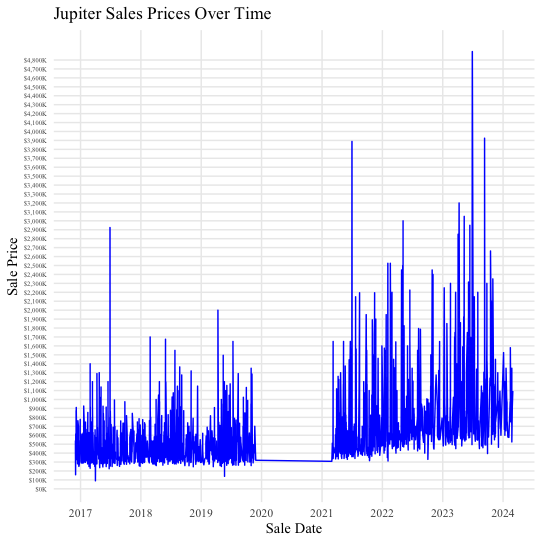
\includegraphics[width=1\linewidth]{jupsalesOT.png}
\caption{This graph visually represents the changes in home sale price in Jupiter, Florida over time between the two sale periods.}
\label{fig:fig1}
\end{figure}

%----------------------------------------
% Figure 2
%----------------------------------------

\begin{figure}[H]
\centering
\bigskip
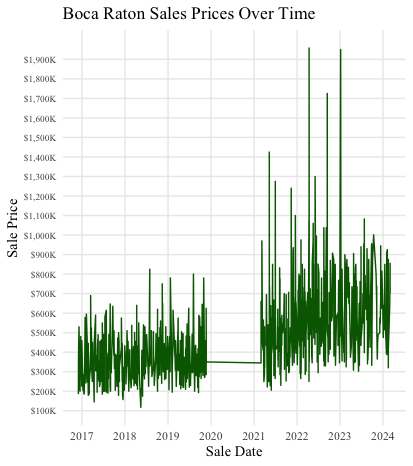
\includegraphics[width=.9\linewidth]{bocasalesOT.png}
\caption{This graph visually represents the changes in home sale price in Boca Raton, Florida over time between the two sale periods.}
\label{fig:fig2}
\end{figure}



\end{document}